\section{Graph-Visualization: \mtbc}
\label{app:chipory}

Processing histories are stored in XML format using {\em GraphML} with some
\alida\ specific extensions as mentioned in Sec.~\ref{subsec:history}.
To display histories we extended
{\em Chisio}\footnote{\href{http://sourceforge.net/projects/chisio}
{http://sourceforge.net/projects/chisio}} to handle the \alida\ specific
extensions, yielding \mtbc.

\subsection{Installation and invocation of \mtbc}

\mtbc is not strictly part of \alida, but supplied as an add-on
at the \alida website%
\footnote{\href{http://www.informatik.uni-halle.de/alida}{http://www.informatik.uni-halle.de/alida}}.
A single zip-file is provided for running \mtbc on Linux systems with 32- or
64-bit as well as on Windows systems. The only difference is one system
dependent jar-file as detailed in the installation instructions provided in the zip archive.
Essentially, all system-independent and one appropriate system-dependent
jar-file have to be included into the CLASSPATH.
Invoke \mtbc, e.g., by
\vspace*{0.5cm}
\begin{code}
  java org.gvt.ChisioMain [directory]
\end{code}

\vspace*{-0.25cm}
The optional directory supplied as an argument denotes the path where
\mtbc starts to browse when reading or writing files.
If omitted, the current working directory is used.

\begin{figure}[ht]
\centerline{{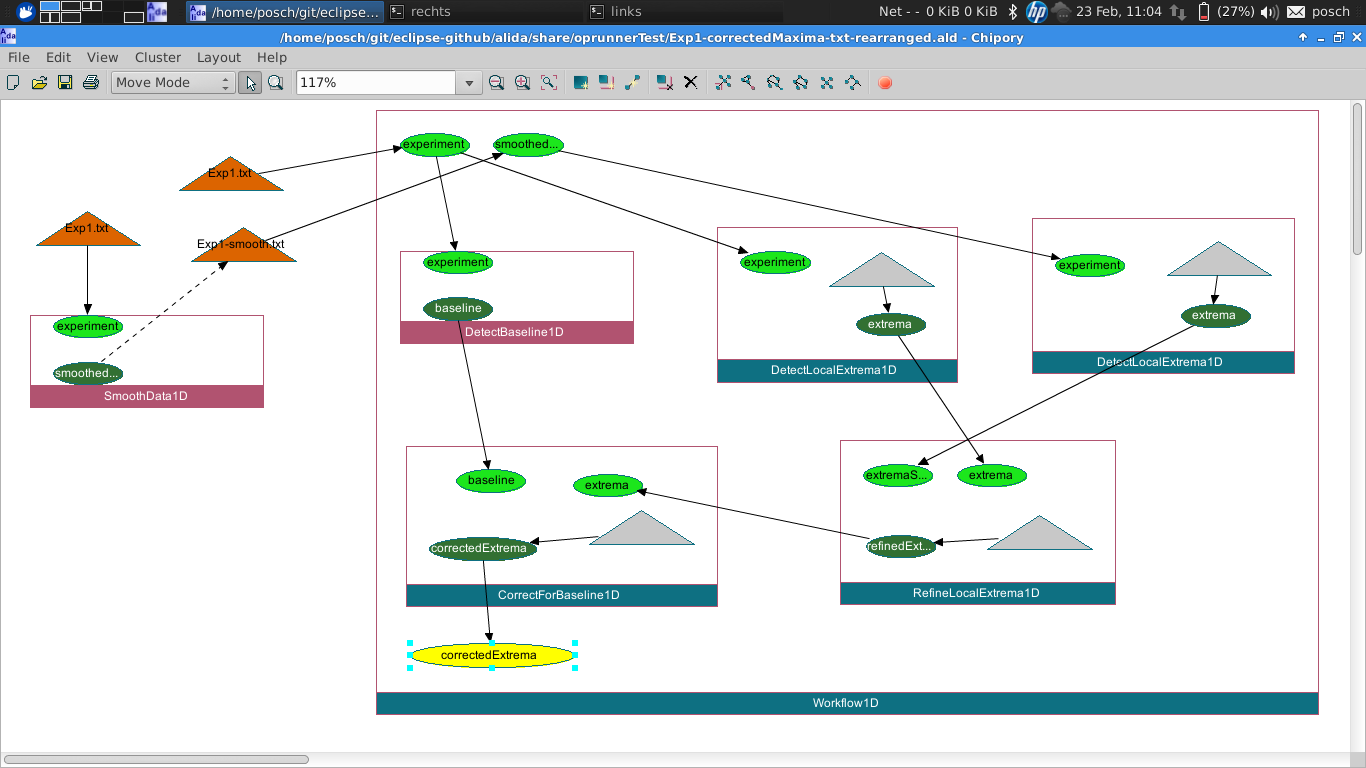
\includegraphics[clip, trim= 10 40 30 90, width=\textwidth]{Exp1-correctedMaxima-txt-rearranged.png}}}
%%{\centerline{{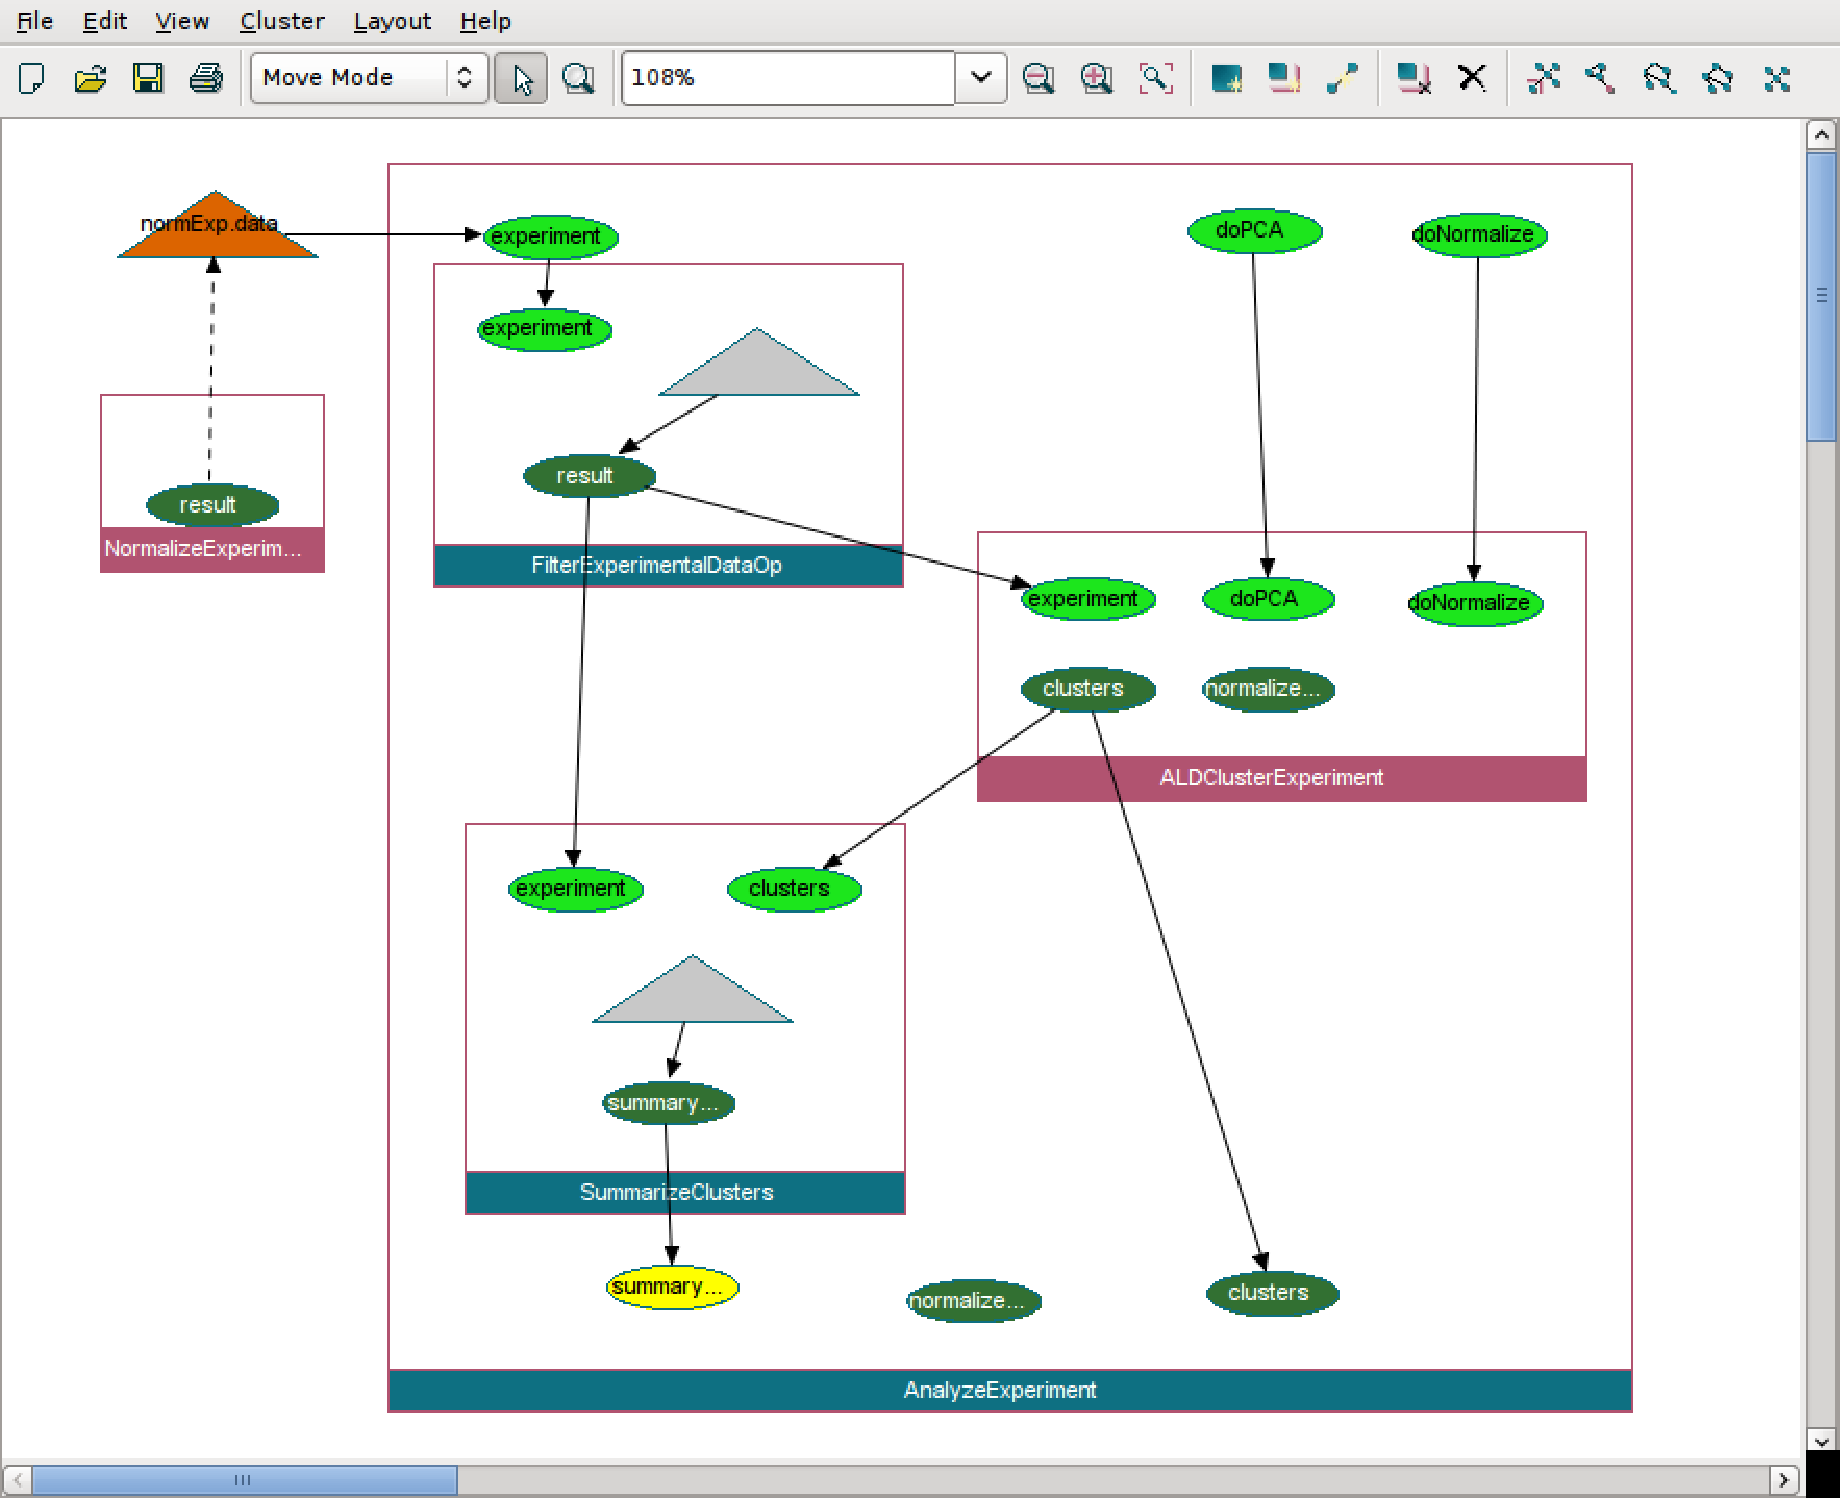
\includegraphics[clip, trim= 0 0 0 0, width=0.85\textwidth]{analyzeData-collapsed-edited}}}}
\caption[Example of a processing graph.]{\label{fig:DAG-repeat}
Example processing graph.
}
\end{figure}

\begin{figure}
\begin{center}
{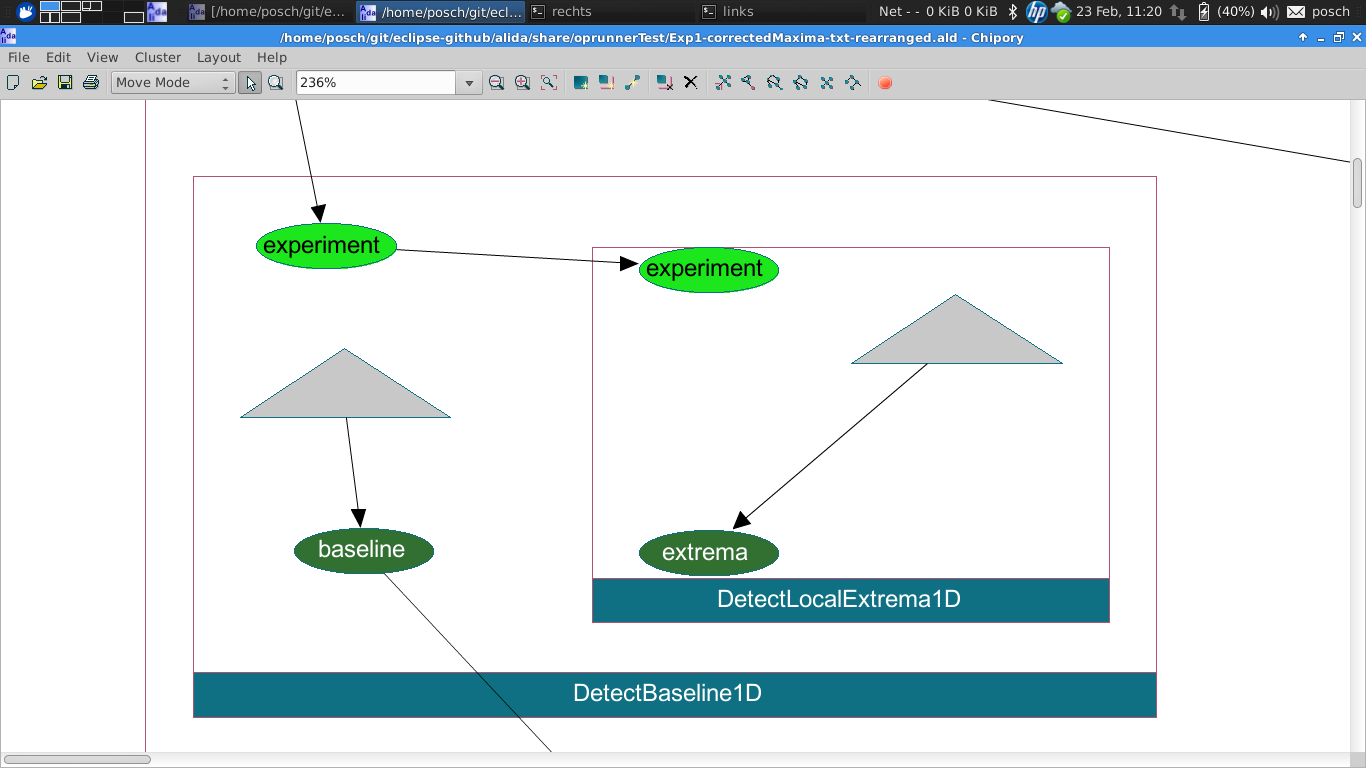
\includegraphics[clip, trim= 180 20 160 140, width=0.4\textwidth]{Exp1-correctedMaxima-txt-uncollapsed.png}}
\caption{\label{fig:exa}Screenshot of \mtbc for a part of the same processing graph as shown in
Fig.~\ref{fig:DAG-repeat}, however, the collapsed instance of the
\icode{DetectBaseline1D} has been uncollapsed.}
\end{center}
\end{figure}

\subsection{Using \mtbc}

\mtbc is based on
{\em Chisio}, a free editing and layout tool for compound or hierarchically
structured graphs. In \mtbc all editing functionality was conserved, however, is not
required for inspecting a processing graph in virtually all cases.
{\em Chisio} offers several automatic layout algorithms where \mtbc chooses
the Sugiyama as default as this is most adequate for the hierarchical graph structure
of processing histories.
In the following we explain a tiny part of {\em Chisio's} functionality and the
extensions supplied by \mtbc.
For more details on {\em Chisio} see the User's manual of {\em Chisio} which is
included in the \mtbc package and also easily found in the web.

In Figure \ref{fig:DAG-repeat} an example processing graph extracted from a data analysis procedure
based on demo operators is shown.
As already described, 
instances of operators are depicted as rectangles, input and output ports as ellipses, and data ports as triangles.
All three types of elements of a processing graph are implemented as
{\em Chisio} nodes. A node may be selected with a left  or right mouse click.
A selected node may be dragged with the left mouse button pressed to manually adjust the
layout.
The size of a node representing operators is automatically adjusted to fit all enclosed
ports and nested operators.

The name of an operator is displayed in a colored area at the bottom of its rectangle.
If an operator node is uncollapsed it is shown in blue, if it is collapsed it is
of dark red.
This is shown in Fig.~\ref{fig:DAG-repeat} 
where the operator \icode{DetectBaseline1D}  
has been collapsed.
A selected operator node may be collapsed or uncollapsed 
via its context menu or by a left double mouse click while pressing down the shift key.
Collapsing makes all enclosed operator and data nodes invisible, thus, only
the ports of a collapsed operator are shown.
If the node is uncollapsed lateron, enclosed nodes are made recursively visible
again, until a collapsed node is encountered.
Uncollapsing additionally invokes the automatic layout algorithm, hence, any manual
layout adjustments applied before are lost.
If we uncollapse the operator \icode{DetectBaseline1D}
as shown in Fig.~\ref{fig:exa}, we can inspect the data processing 
accomplished within this operator.

If a data port represents data read from file,
the triangle is tagged by a string and colored orange.
%%If the
%%data object extends the class \icode{ALDData} this string gives the filename
%%the data was read from.
As the data read from file \icode{'Exp1-smooth.txt'}
has a processing graph associated,
this history is also included into the processing graph and 
connected by a dashed edge.
This history was written to the file \icode{'Exp1-smooth.txt.ald'} by previous
processing using \alida.

%%From this processing history we find
%%that the median operation has been applied to an image \icode{foo.pgm}
%%which in turn had no associated history.

\begin{figure}
\begin{center}
{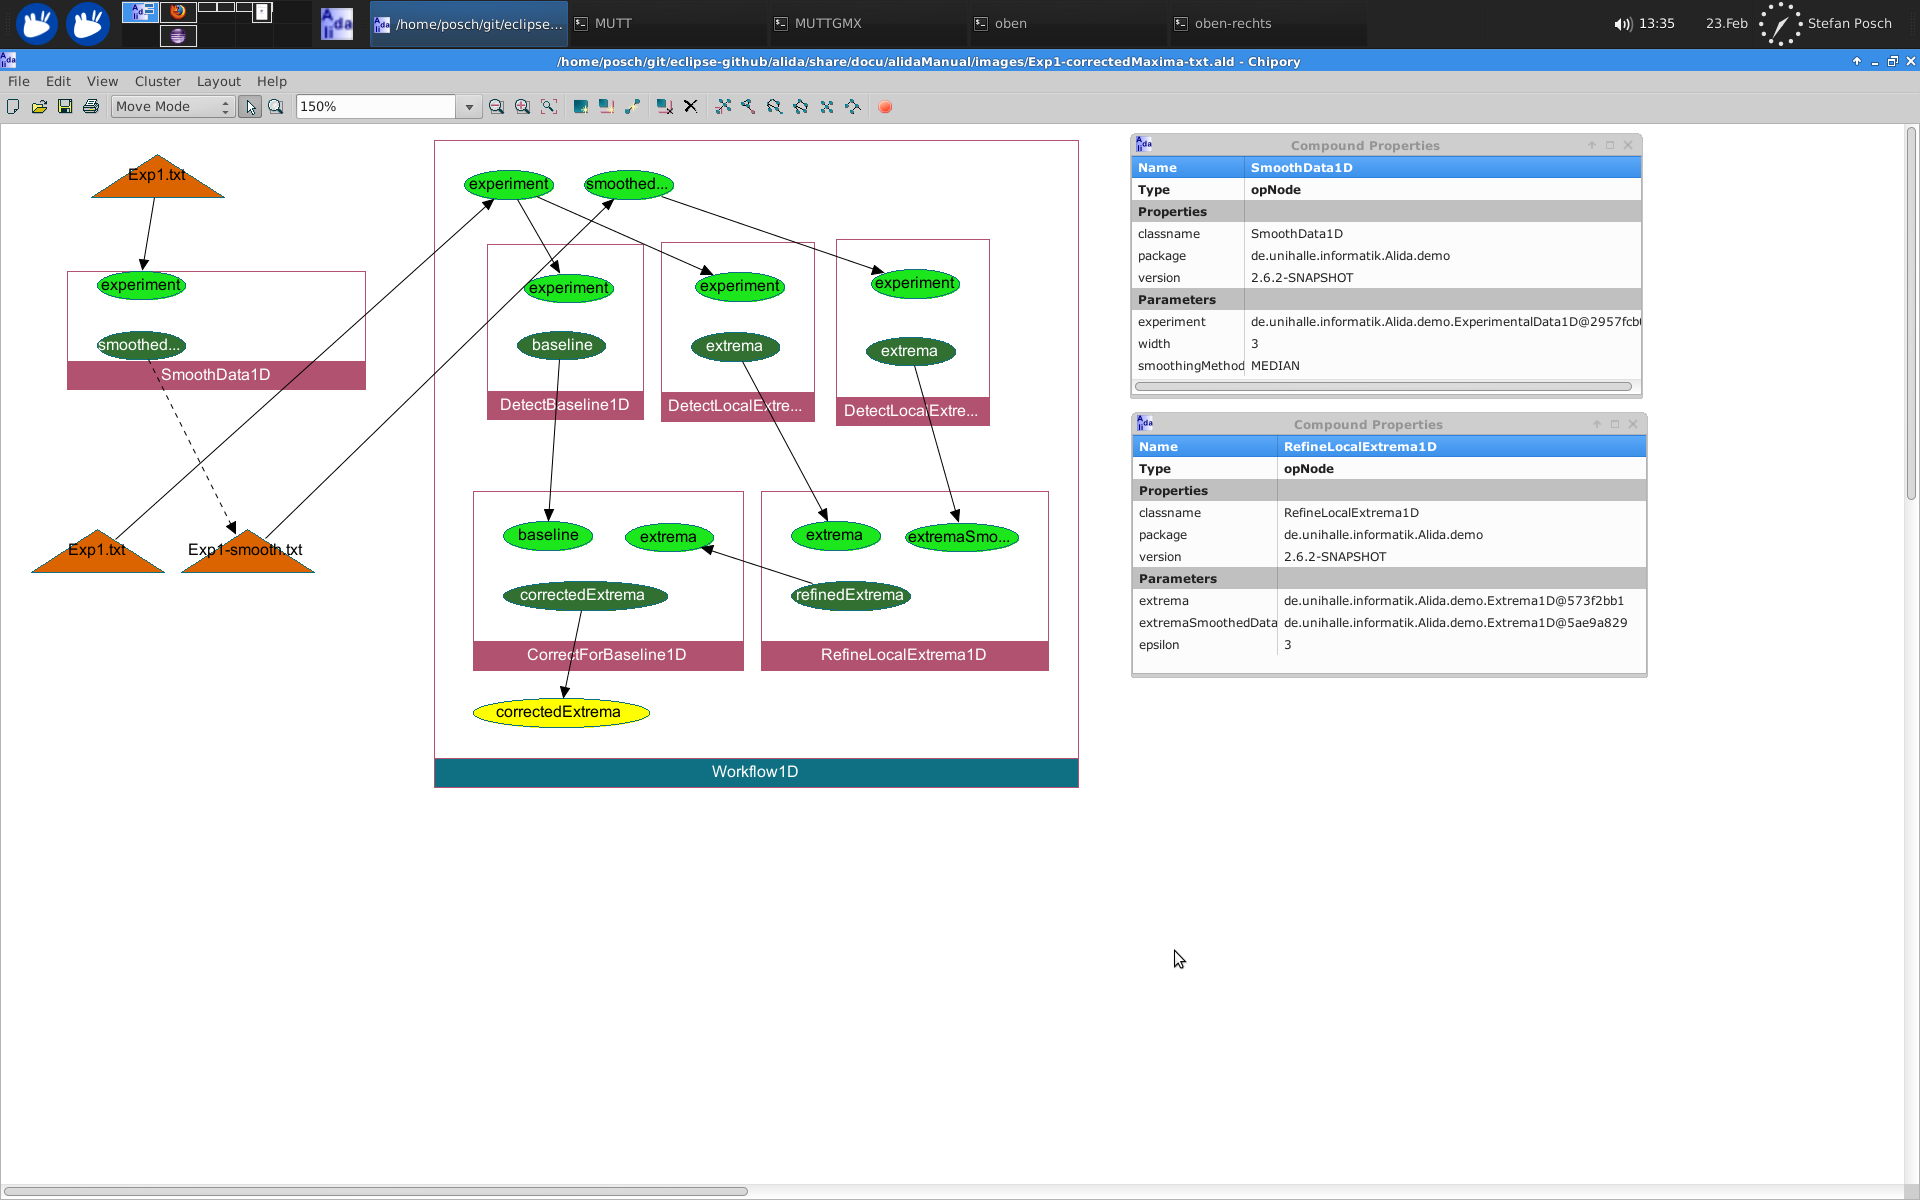
\includegraphics[clip,trim=10 380 190 130,width=\textwidth]{Exp1-correctedMaxima-txt-withPorperties.png}}
\caption{\label{fig:exa1}Screenshot of \mtbc with details for the operators
\icode{SmoothData1D} and \icode{RefineLocalExtrema1D}.
}
\end{center}
\end{figure}


Input and output ports are generally displayed with light and 
dark green ellipses, respectively. 
The single exception
is the port for which the processing graph was constructed, which is depicted in
yellow.
In our example this is the output port \icode{'correctedExtrema'} of the
operator \icode{CorrectForBaseline1D}.

More details for operators and ports may be inspected using the \textit{Object properties}
of {\em Chisio's} nodes.
These are displayed in a separate window which
for the selected node can be popped up using the context menu.
The context menu is activated by a right mouse click.
Alternatively the object properties window can be popped up by a double left mouse click.

Information displayed includes:
\begin{itemize}\itemseparation{0.1em}
\item	name of the operator or port
\item	type of the node, e.g., \icode{opNode} for operators
\item	for operators the parameter values at time of invocation
\item	for input and output ports the Java class of the object as it was passed
into the operator along with the explanatory text of this port
\item	for output ports the properties of the object
	given when passed out of the operator, if it is of type \icode{ALDData}.
\end{itemize}
In Fig.~\ref{fig:exa1} this is shown for the operators
\icode{SmoothData1D} and \icode{RefineLocalExtrema1D}.



